\documentclass[12pt,a4paper]{report}

\usepackage[utf8]{vietnam}
\usepackage{amsmath, amsthm, amssymb,latexsym,amscd,amsfonts,enumerate}
\usepackage{color, fancyhdr, graphicx, wrapfig}
\usepackage{listings}

\definecolor{dkgreen}{rgb}{0,0.6,0}
\definecolor{gray}{rgb}{0.5,0.5,0.5}
\definecolor{mauve}{rgb}{0.58,0,0.82}
\lstset{frame=tb,
  language=SQL,
  aboveskip=3mm,
  belowskip=3mm,
  showstringspaces=false,
  columns=flexible,
  basicstyle={\small\ttfamily},
  numbers=none,
  numberstyle=\tiny\color{gray},
  keywordstyle=\color{blue},
  commentstyle=\color{dkgreen},
  stringstyle=\color{mauve},
  breaklines=true,
  breakatwhitespace=true,
  tabsize=3
}


\begin{document}
\fontsize{13pt}{18pt}\selectfont
\section{Truy vấn dữ liệu}
\subsection{MulticarAddress}

	{\bf Yêu cầu truy vấn:} Tìm ra đại diện của hộ gia đình đang trong thời hạn hưởng chính sách bảo hiểm. Hộ gia đình được xác định bởi nhóm các khách hàng có cùng AddressId(số lượng lớn hơn 1).
	
	{\bf Câu lệnh:}
	\begin{lstlisting}
		USE nguyenhieu;
		SELECT
			CustomerID,
    		Title,
    		FName AS FirstName,
    		LName AS LastName,
    		EmailAddress,
    		TelephoneNumber,
    		VehicleReg,
    		HouseNumber,
    		PostCode,
    		Price AS 'Price($)'
		From customer
		LEFT JOIN policy ON customer.ID = policy.CustomerID
		LEFT JOIN address ON customer.AddressID = address.ID
		WHERE CURDATE() BETWEEN PolicyStartDate AND PolicyEndDate
		AND AddressID IN (
			SELECT customer.AddressID
			FROM customer
			GROUP BY AddressID
			HAVING COUNT(AddressID) > 1
		)
		ORDER BY CustomerID;
	\end{lstlisting}

	{\bf Kết quả dữ liệu:}
	\\
	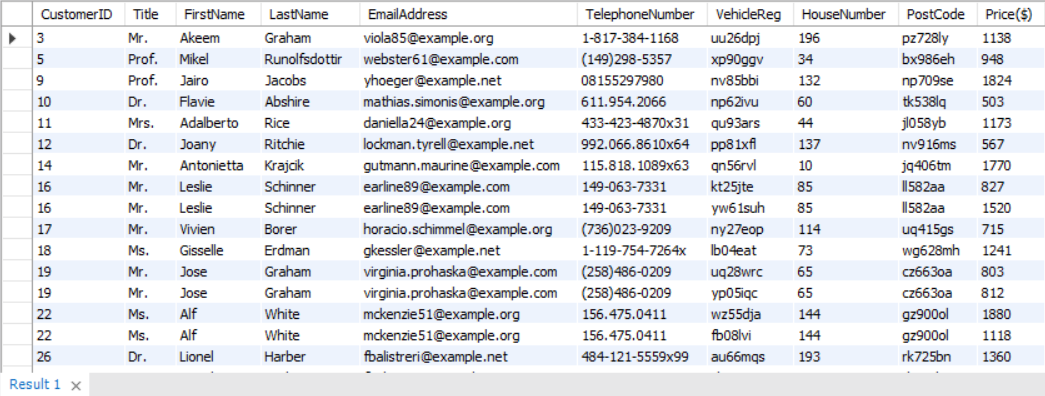
\includegraphics[width=\linewidth]{MulticarAddress}
\subsection{MultiPolicyBenefits}

	{\bf Yêu cầu truy vấn:} Lấy ra danh sách những chính sách bảo hiểm có cùng hiệu lực ở thời điểm hiện tại của từng khách hàng.

	{\bf Câu lệnh:}
	\begin{lstlisting}
		SELECT 
			x.pol1 AS PolicyID,
    		x.cus1 AS CustomerID,
    		x.pol2 AS PolicyID2,
    		x.cus2 AS CustomerID2
		FROM(
    		SELECT
				P1.ID AS pol1,
        		P1.CustomerID AS cus1,
        		P1.PolicyStartDate,
        		P1.PolicyEndDate,
        		P2.CustomerID AS cus2,
        		P2.ID AS pol2
    		FROM policy AS P1, policy AS P2
    		WHERE P1.ID < P2.ID
    		AND P1.PolicyStartDate BETWEEN P2.PolicyStartDate AND P2.PolicyEndDate
    		OR P1.PolicyEndDate BETWEEN P2.PolicyStartDate AND P2.PolicyEndDate
		)AS X
		WHERE pol1 <> pol2
		AND cus1 = cus2
		AND CURDATE() BETWEEN X.PolicyStartDate AND X.PolicyEndDate;
	\end{lstlisting}

	{\bf Kết quả dữ liệu:}
	\\
	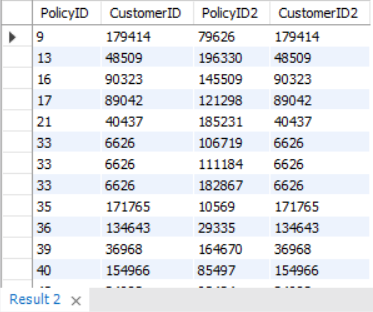
\includegraphics[width=\linewidth]{MultiPolicyBenefits}
	
\subsection{PriceCalculation}
	{\bf Yêu cầu truy vấn:} Tính chi phí bảo hiểm của tất cả các chính sách.
	
	{\bf Câu lệnh:}
	\begin{lstlisting}
		SELECT DISTINCT
			PolicyID,
    		BasePrice,
    		Metric,
    		ROUND(((Baseprice/100*metric)/100)*(`PaymentTypePercentageChange(%)`+100),2) as 'totalPrice($)'
FROM (
			SELECT DISTINCT 
				PolicyID,
				(x.VehicleValue / 100) * 25 AS BasePrice,
        		(EngineClass + OccupationClass + AgeClass + VehicleModClass + MedicalConditionClass)+100 AS Metric,
        		`PaymentTypePercentageChange(%)`
			FROM (
				SELECT
					policy.ID AS PolicyID,
            		Fname,
            		VehicleReg,
            		VehicleValue,
            		CASE
						WHEN EngineCC BETWEEN 1000 AND 1199 THEN 0
						WHEN EngineCC BETWEEN 1200 AND 1399 THEN 10
						WHEN EngineCC BETWEEN 1400 AND 1599 THEN 20
						WHEN EngineCC BETWEEN 1600 AND 1799 THEN 30
						WHEN EngineCC BETWEEN 1800 AND 1999 THEN 40
						WHEN EngineCC BETWEEN 2000 AND 2199 THEN 50
						WHEN EngineCC BETWEEN 2200 AND 2399 THEN 60
						WHEN EngineCC BETWEEN 2400 AND 2599 THEN 70
						WHEN EngineCC BETWEEN 2600 AND 2799 THEN 80
						WHEN EngineCC BETWEEN 2800 AND 2999 THEN 90
						WHEN EngineCC BETWEEN 3000 AND 3199 THEN 100
						WHEN EngineCC BETWEEN 3200 AND 3399 THEN 110
						WHEN EngineCC BETWEEN 3400 AND 3599 THEN 120
						WHEN EngineCC BETWEEN 3600 AND 3799 THEN 130
						WHEN EngineCC BETWEEN 3800 AND 3999 THEN 140
                		ELSE 200
					END AS EngineClass,
            		CASE
						WHEN FLOOR(DATEDIFF(PolicyStartDate, DOB) / 365) <= 16 THEN 30
						WHEN FLOOR(DATEDIFF(PolicyStartDate, DOB) / 365) BETWEEN 17 AND 19 THEN 30
						WHEN FLOOR(DATEDIFF(PolicyStartDate, DOB) / 365) BETWEEN 20 AND 25 THEN 20
						WHEN FLOOR(DATEDIFF(PolicyStartDate, DOB) / 365) BETWEEN 26 AND 29 THEN 10
						WHEN FLOOR(DATEDIFF(PolicyStartDate, DOB) / 365) BETWEEN 30 AND 35 THEN 0
						WHEN FLOOR(DATEDIFF(PolicyStartDate, DOB) / 365) BETWEEN 35 AND 39 THEN -10
						WHEN FLOOR(DATEDIFF(PolicyStartDate, DOB) / 365) BETWEEN 40 AND 49 THEN -20
						WHEN FLOOR(DATEDIFF(PolicyStartDate, DOB) / 365) BETWEEN 50 AND 59 THEN -30
						WHEN FLOOR(DATEDIFF(PolicyStartDate, DOB) / 365) BETWEEN 60 AND 90 THEN 20
                		ELSE 0
            		END AS AgeClass,
            		Modifier  AS OccupationClass,
            		CASE
						WHEN SUM(Points) > 1 THEN SUM(Points)
                		ELSE 0
					END AS VehicleModClass,
            		CASE
						WHEN MedicalCondition = 'No' THEN 0
						WHEN MedicalCondition = 'Yes' THEN 10
						ELSE 20
            		END AS MedicalConditionClass,
            		CASE
						WHEN PaymentType = 'Annual' THEN 0
						WHEN PaymentType = 'Monthly' THEN 20
						ELSE 10
					END AS 'PaymentTypePercentageChange(%)'
				FROM vehicle
					JOIN policy ON vehicle.Registration = policy.VehicleReg
					JOIN customer ON policy.CustomerID = customer.ID
					JOIN occupation ON customer.Occupation = occupation.ID
					LEFT JOIN mod_vehicle ON vehicle.Registration = mod_vehicle.Reg
					LEFT JOIN `mod` ON mod_vehicle.VehicleMod = `mod`.ID
				GROUP BY PolicyID
    		) AS X
		) AS Y
		WHERE PolicyID BETWEEN 10000 AND 20000;
	\end{lstlisting}
	
	{\bf Kết quả dữ liệu:}
	\\
	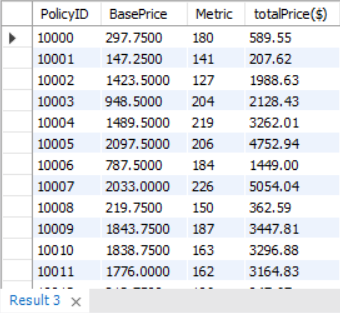
\includegraphics[width=\linewidth]{PriceCalculation}
	
\subsection{ProfitsByFiscalYear}
	{\bf Yêu cầu truy vấn:} Nhóm theo các năm, số tiền phải trả cho khách hàng và lợi nhuận.
	
	{\bf Câu lệnh:}
	\begin{lstlisting}
		SELECT
			sales.FinancialYear,
			sales.Gross,
    		CASE
				WHEN expenses.expense IS NULL THEN 0
        		ELSE expenses.expense
			END AS AmountSpentOnClaims,
    		CASE
				WHEN sales.gross - expenses.expense IS NULL THEN sales.gross
        		ELSE sales.gross - expenses.expense
			END AS 'Profit/Loss ($)'
		FROM (
			SELECT
				CASE
					WHEN MONTH(policy.PolicyStartDate) >= 6
						THEN concat(YEAR(policy.PolicyStartDate), ' to ', YEAR(policy.PolicyStartDate) + 1)
					ELSE concat(YEAR(policy.PolicyStartDate) - 1, ' to ', YEAR(policy.PolicyStartDate))
				END AS FinancialYear,
        		SUM(policy.Price) AS Gross
			FROM policy
			GROUP BY FinancialYear
		) AS sales
		LEFT JOIN (
			SELECT 
				CASE
					WHEN MONTH(claim.DatePaid) >= 6
						THEN CONCAT(YEAR(claim.DatePaid), ' to ',YEAR(claim.DatePaid) + 1)
					ELSE CONCAT(YEAR(claim.DatePaid)-1,' to ', YEAR(claim.DatePaid))
				END AS FinancialYear,
        		SUM(claim.AmountPaidOut) AS expense
			FROM claim
    		GROUP BY FinancialYear
    		HAVING FinancialYear IS NOT NULL
		) AS expenses ON expenses.FinancialYear = sales.FinancialYear;
	\end{lstlisting}
	
	{\bf Kết quả dữ liệu:}
	\\
	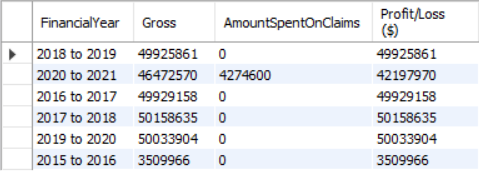
\includegraphics[width=\linewidth]{ProfitsByFiscalYear}
	
\subsection{UpcomingRenewals}
	{\bf Yêu cầu truy vấn:} Số ngày còn lại cho đến hạn cuối của chính sách bảo hiểm của mỗi khách hàng
	
	
	{\bf Câu lệnh:}
	\begin{lstlisting}
		SELECT
			Title,
    		FName AS 'First Name',
   			LName AS 'Last Name',
    		EmailAddress,
    		TelephoneNumber,
    		DATE_FORMAT(CURDATE(), '%d/%m/%Y') AS 'Today Date',
    		DATE_FORMAT(PolicyEndDate, '%d/%m/%Y') AS 'Policy End Date',
    		DATEDIFF(PolicyEndDate, CURDATE()) AS 'Days left',
			policy.ID AS PolicyID,
    		VehicleReg
		FROM customer
		LEFT JOIN policy ON customer.ID = policy.CustomerID
		WHERE PolicyEndDate BETWEEN CURDATE() AND DATE_ADD(NOW(), INTERVAL 30 DAY);
	\end{lstlisting}

	{\bf Kết quả dữ liệu:}
	\\
	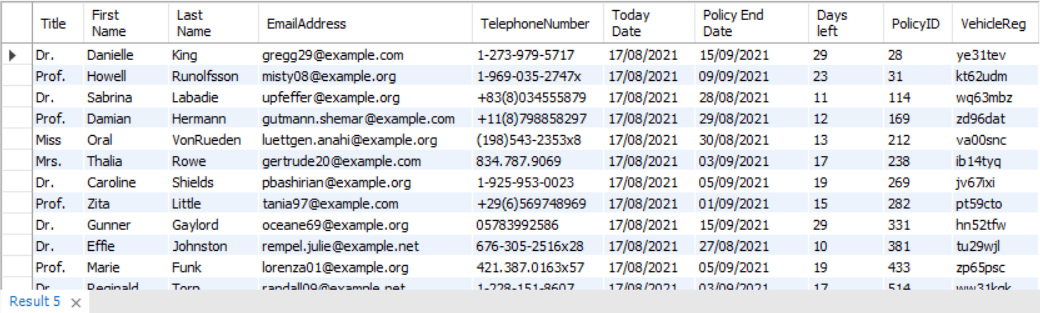
\includegraphics[width=\linewidth]{UpcomingRenewals}
	
\section{Tối ưu truy vấn}
\subsection{Index}
	{\bf Câu lệnh truy vấn:}
	\begin{lstlisting}
	SELECT
		policy.ID AS PolicyID,
		Fname,
		VehicleReg,
		VehicleValue,
	CASE
		WHEN EngineCC BETWEEN 1000 AND 1199 THEN 0
		WHEN EngineCC BETWEEN 1200 AND 1399 THEN 10
		WHEN EngineCC BETWEEN 1400 AND 1599 THEN 20
		WHEN EngineCC BETWEEN 1600 AND 1799 THEN 30
		WHEN EngineCC BETWEEN 1800 AND 1999 THEN 40
		WHEN EngineCC BETWEEN 2000 AND 2199 THEN 50
		WHEN EngineCC BETWEEN 2200 AND 2399 THEN 60
		WHEN EngineCC BETWEEN 2400 AND 2599 THEN 70
		WHEN EngineCC BETWEEN 2600 AND 2799 THEN 80
		WHEN EngineCC BETWEEN 2800 AND 2999 THEN 90
		WHEN EngineCC BETWEEN 3000 AND 3199 THEN 100
		WHEN EngineCC BETWEEN 3200 AND 3399 THEN 110
		WHEN EngineCC BETWEEN 3400 AND 3599 THEN 120
		WHEN EngineCC BETWEEN 3600 AND 3799 THEN 130
		WHEN EngineCC BETWEEN 3800 AND 3999 THEN 140
		ELSE 200
	END AS EngineClass,
	CASE
		WHEN FLOOR(DATEDIFF(PolicyStartDate, DOB) / 365) <= 16 THEN 30
		WHEN FLOOR(DATEDIFF(PolicyStartDate, DOB) / 365) BETWEEN 17 AND 19 THEN 30
		WHEN FLOOR(DATEDIFF(PolicyStartDate, DOB) / 365) BETWEEN 20 AND 25 THEN 20
		WHEN FLOOR(DATEDIFF(PolicyStartDate, DOB) / 365) BETWEEN 26 AND 29 THEN 10
		WHEN FLOOR(DATEDIFF(PolicyStartDate, DOB) / 365) BETWEEN 30 AND 35 THEN 0
		WHEN FLOOR(DATEDIFF(PolicyStartDate, DOB) / 365) BETWEEN 35 AND 39 THEN -10
		WHEN FLOOR(DATEDIFF(PolicyStartDate, DOB) / 365) BETWEEN 40 AND 49 THEN -20
		WHEN FLOOR(DATEDIFF(PolicyStartDate, DOB) / 365) BETWEEN 50 AND 59 THEN -30
		WHEN FLOOR(DATEDIFF(PolicyStartDate, DOB) / 365) BETWEEN 60 AND 90 THEN 20
		ELSE 0
	END AS AgeClass,
	Modifier  AS OccupationClass,
	CASE
		WHEN SUM(Points) > 1 THEN SUM(Points)
		ELSE 0
	END AS VehicleModClass,
	CASE
		WHEN MedicalCondition = 'No' THEN 0
		WHEN MedicalCondition = 'Yes' THEN 10
		ELSE 20
	END AS MedicalConditionClass,
	CASE
		WHEN PaymentType = 'Annual' THEN 0
		WHEN PaymentType = 'Monthly' THEN 20
		ELSE 10
	END AS 'PaymentTypePercentageChange(%)'
FROM vehicle
	JOIN policy ON vehicle.Registration = policy.VehicleReg
	JOIN customer ON policy.CustomerID = customer.ID
	JOIN occupation ON customer.Occupation = occupation.ID
	LEFT JOIN mod_vehicle ON vehicle.Registration = mod_vehicle.Reg
	LEFT JOIN `mod` ON mod_vehicle.VehicleMod = `mod`.ID
WHERE
	VehicleValue BETWEEN 5000 AND 8000
GROUP BY PolicyID;
	\end{lstlisting}
	
	{\bf Trước khi thêm index:}
	\\
	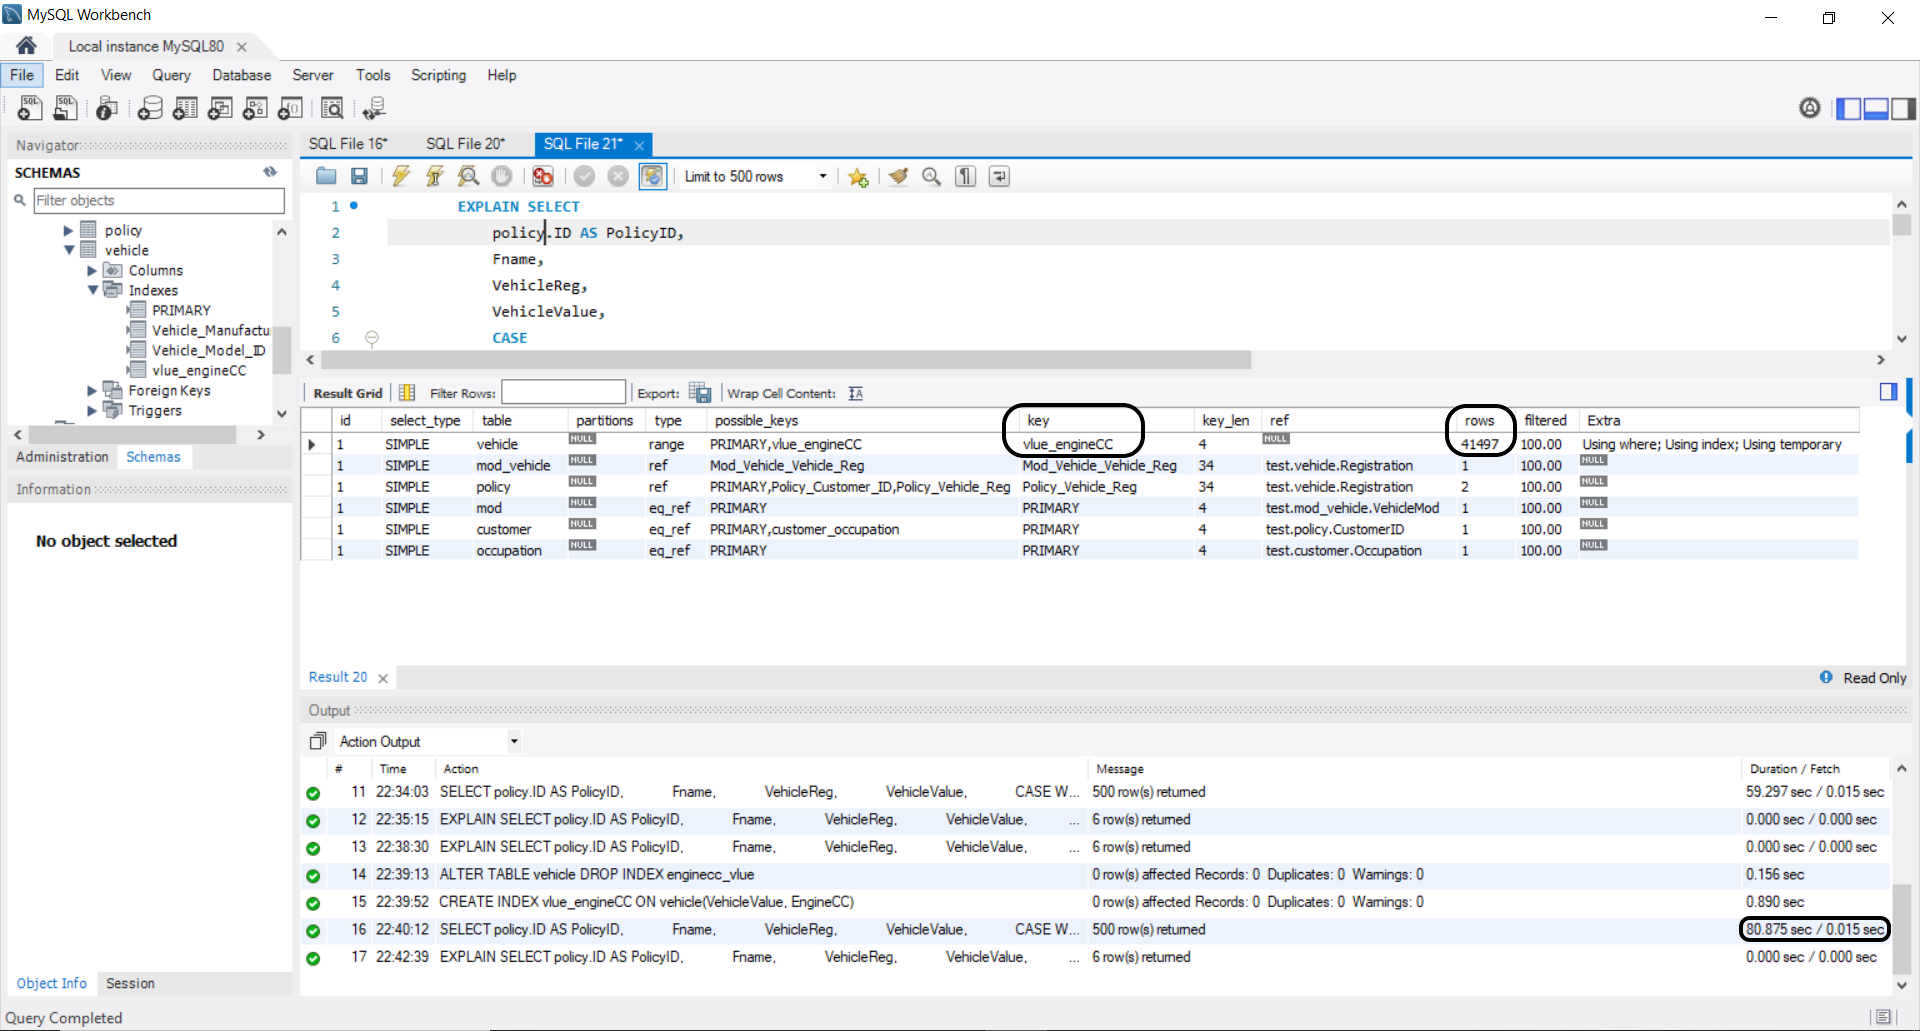
\includegraphics[width=\linewidth]{BeforeIndexing}
	
	{\bf Sau khi thêm index:}
	\\
	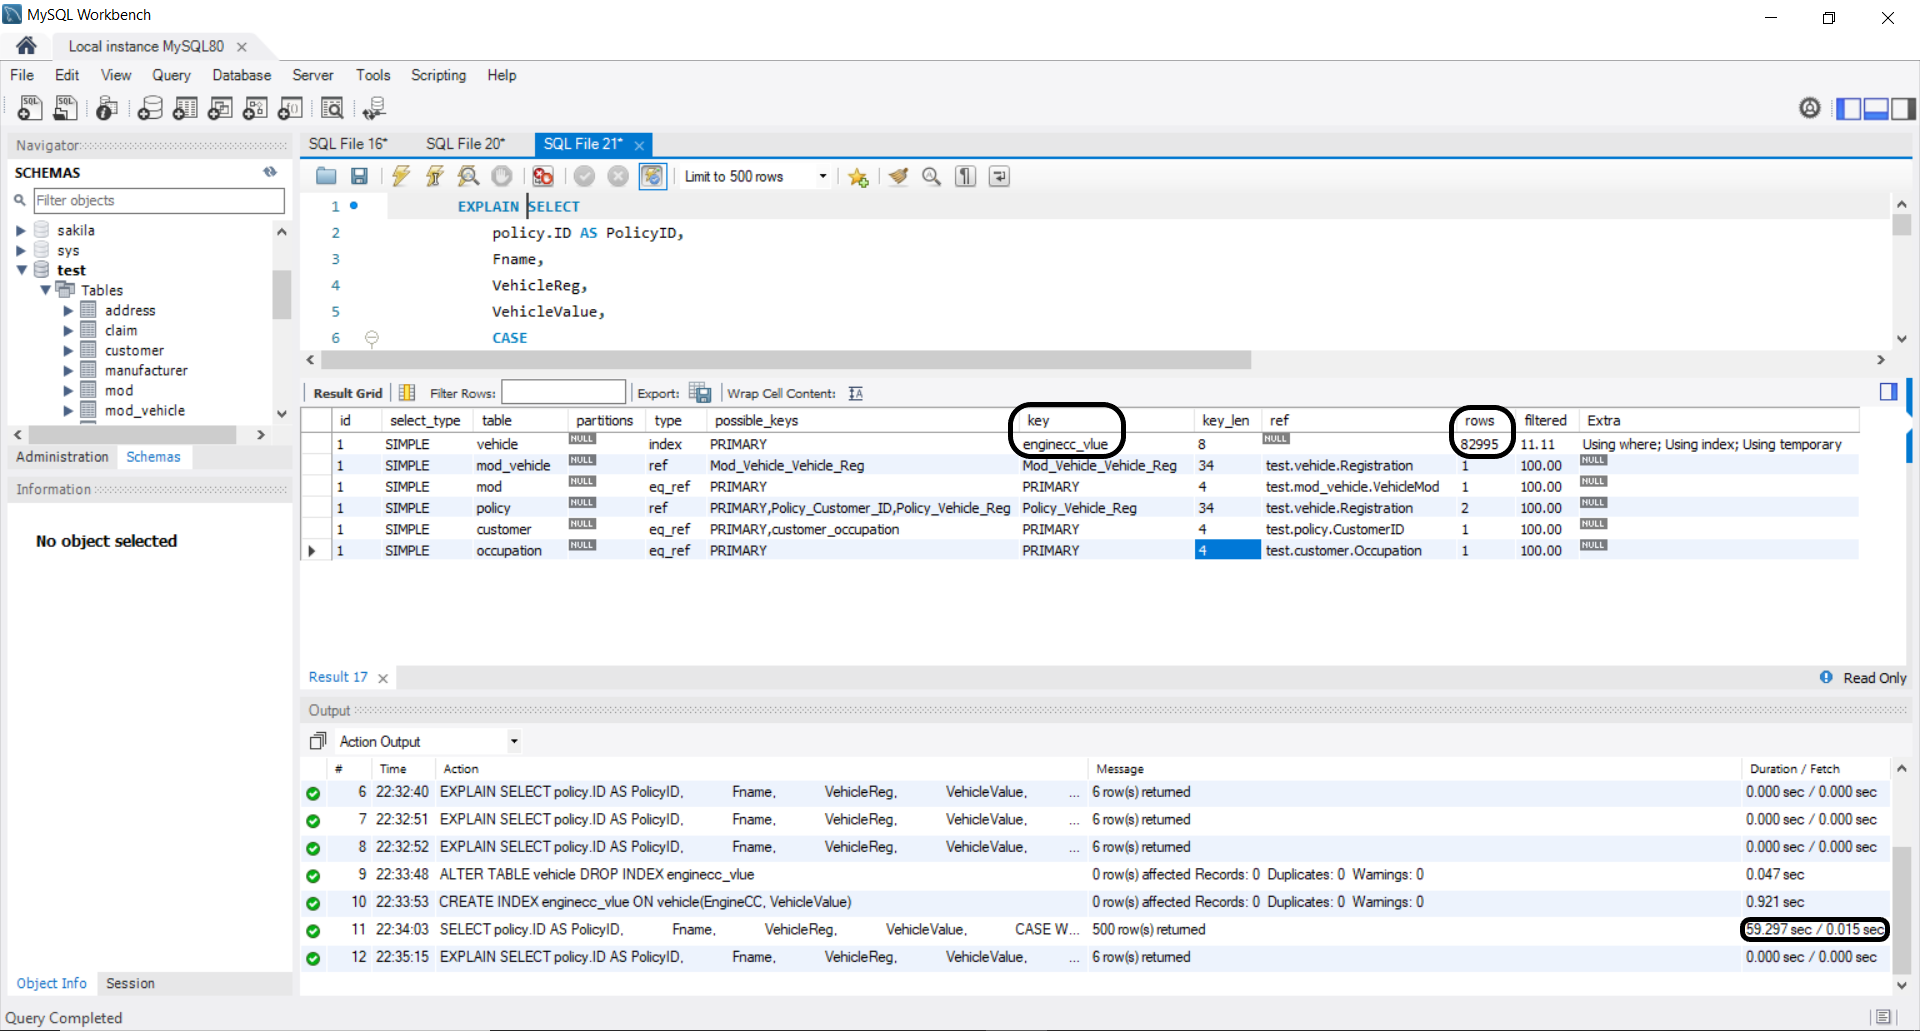
\includegraphics[width=\linewidth]{AfterIndexing}
\subsection{Partition}
	{\bf Câu lệnh truy vấn}
	\begin{lstlisting}
		EXPLAIN SELECT 
			PolicyID,
    		FName,
    		PolicyStartDate,
    		YearsNCB
		FROM part_Table
			JOIN policy ON part_table.PolicyID = policy.ID
		WHERE EngineClass IN (10, 50, 80, 140);
	\end{lstlisting}
	
	{\bf Bảng để partition:}
	\begin{lstlisting}
CREATE TABLE part_Table
	SELECT
		policy.ID AS PolicyID,
		Fname,
		VehicleReg,
		VehicleValue,
		CASE
			WHEN EngineCC BETWEEN 1000 AND 1199 THEN 0
			WHEN EngineCC BETWEEN 1200 AND 1399 THEN 10
			WHEN EngineCC BETWEEN 1400 AND 1599 THEN 20
			WHEN EngineCC BETWEEN 1600 AND 1799 THEN 30
			WHEN EngineCC BETWEEN 1800 AND 1999 THEN 40
			WHEN EngineCC BETWEEN 2000 AND 2199 THEN 50
			WHEN EngineCC BETWEEN 2200 AND 2399 THEN 60
			WHEN EngineCC BETWEEN 2400 AND 2599 THEN 70
			WHEN EngineCC BETWEEN 2600 AND 2799 THEN 80
			WHEN EngineCC BETWEEN 2800 AND 2999 THEN 90
			WHEN EngineCC BETWEEN 3000 AND 3199 THEN 100
			WHEN EngineCC BETWEEN 3200 AND 3399 THEN 110
			WHEN EngineCC BETWEEN 3400 AND 3599 THEN 120
			WHEN EngineCC BETWEEN 3600 AND 3799 THEN 130
			WHEN EngineCC BETWEEN 3800 AND 3999 THEN 140
			ELSE 200
		END AS EngineClass,
		CASE
			WHEN FLOOR(DATEDIFF(PolicyStartDate, DOB) / 365) <= 16 THEN 30
			WHEN FLOOR(DATEDIFF(PolicyStartDate, DOB) / 365) BETWEEN 17 AND 19 THEN 30
			WHEN FLOOR(DATEDIFF(PolicyStartDate, DOB) / 365) BETWEEN 20 AND 25 THEN 20
			WHEN FLOOR(DATEDIFF(PolicyStartDate, DOB) / 365) BETWEEN 26 AND 29 THEN 10
			WHEN FLOOR(DATEDIFF(PolicyStartDate, DOB) / 365) BETWEEN 30 AND 35 THEN 0
			WHEN FLOOR(DATEDIFF(PolicyStartDate, DOB) / 365) BETWEEN 35 AND 39 THEN -10
			WHEN FLOOR(DATEDIFF(PolicyStartDate, DOB) / 365) BETWEEN 40 AND 49 THEN -20
			WHEN FLOOR(DATEDIFF(PolicyStartDate, DOB) / 365) BETWEEN 50 AND 59 THEN -30
			WHEN FLOOR(DATEDIFF(PolicyStartDate, DOB) / 365) BETWEEN 60 AND 90 THEN 20
			ELSE 0
		END AS AgeClass,
		Modifier  AS OccupationClass,
		CASE
			WHEN SUM(Points) > 1 THEN SUM(Points)
			ELSE 0
		END AS VehicleModClass,
		CASE
			WHEN MedicalCondition = 'No' THEN 0
			WHEN MedicalCondition = 'Yes' THEN 10
			ELSE 20
		END AS MedicalConditionClass,
		CASE
			WHEN PaymentType = 'Annual' THEN 0
			WHEN PaymentType = 'Monthly' THEN 20
			ELSE 10
		END AS 'PaymentTypePercentageChange(%)'
	FROM vehicle
		JOIN policy ON vehicle.Registration = policy.VehicleReg
		JOIN customer ON policy.CustomerID = customer.ID
		JOIN occupation ON customer.Occupation = occupation.ID
		LEFT JOIN mod_vehicle ON vehicle.Registration = mod_vehicle.Reg
		LEFT JOIN `mod` ON mod_vehicle.VehicleMod = `mod`.ID
	GROUP BY PolicyID;
	\end{lstlisting}
	
	{\bf Câu lệnh partition:}
	\begin{lstlisting}
		ALTER TABLE part_Table
		PARTITION BY RANGE (EngineClass) (
			PARTITION p00 VALUES LESS THAN (20),
			PARTITION p01 VALUES LESS THAN (40),
			PARTITION p02 VALUES LESS THAN (60),
			PARTITION p03 VALUES LESS THAN (80),
			PARTITION p04 VALUES LESS THAN (100),
			PARTITION p05 VALUES LESS THAN (120),
			PARTITION p06 VALUES LESS THAN MAXVALUE
		);
	\end{lstlisting}

	{\bf Trước khi thêm partition:}
	\\
	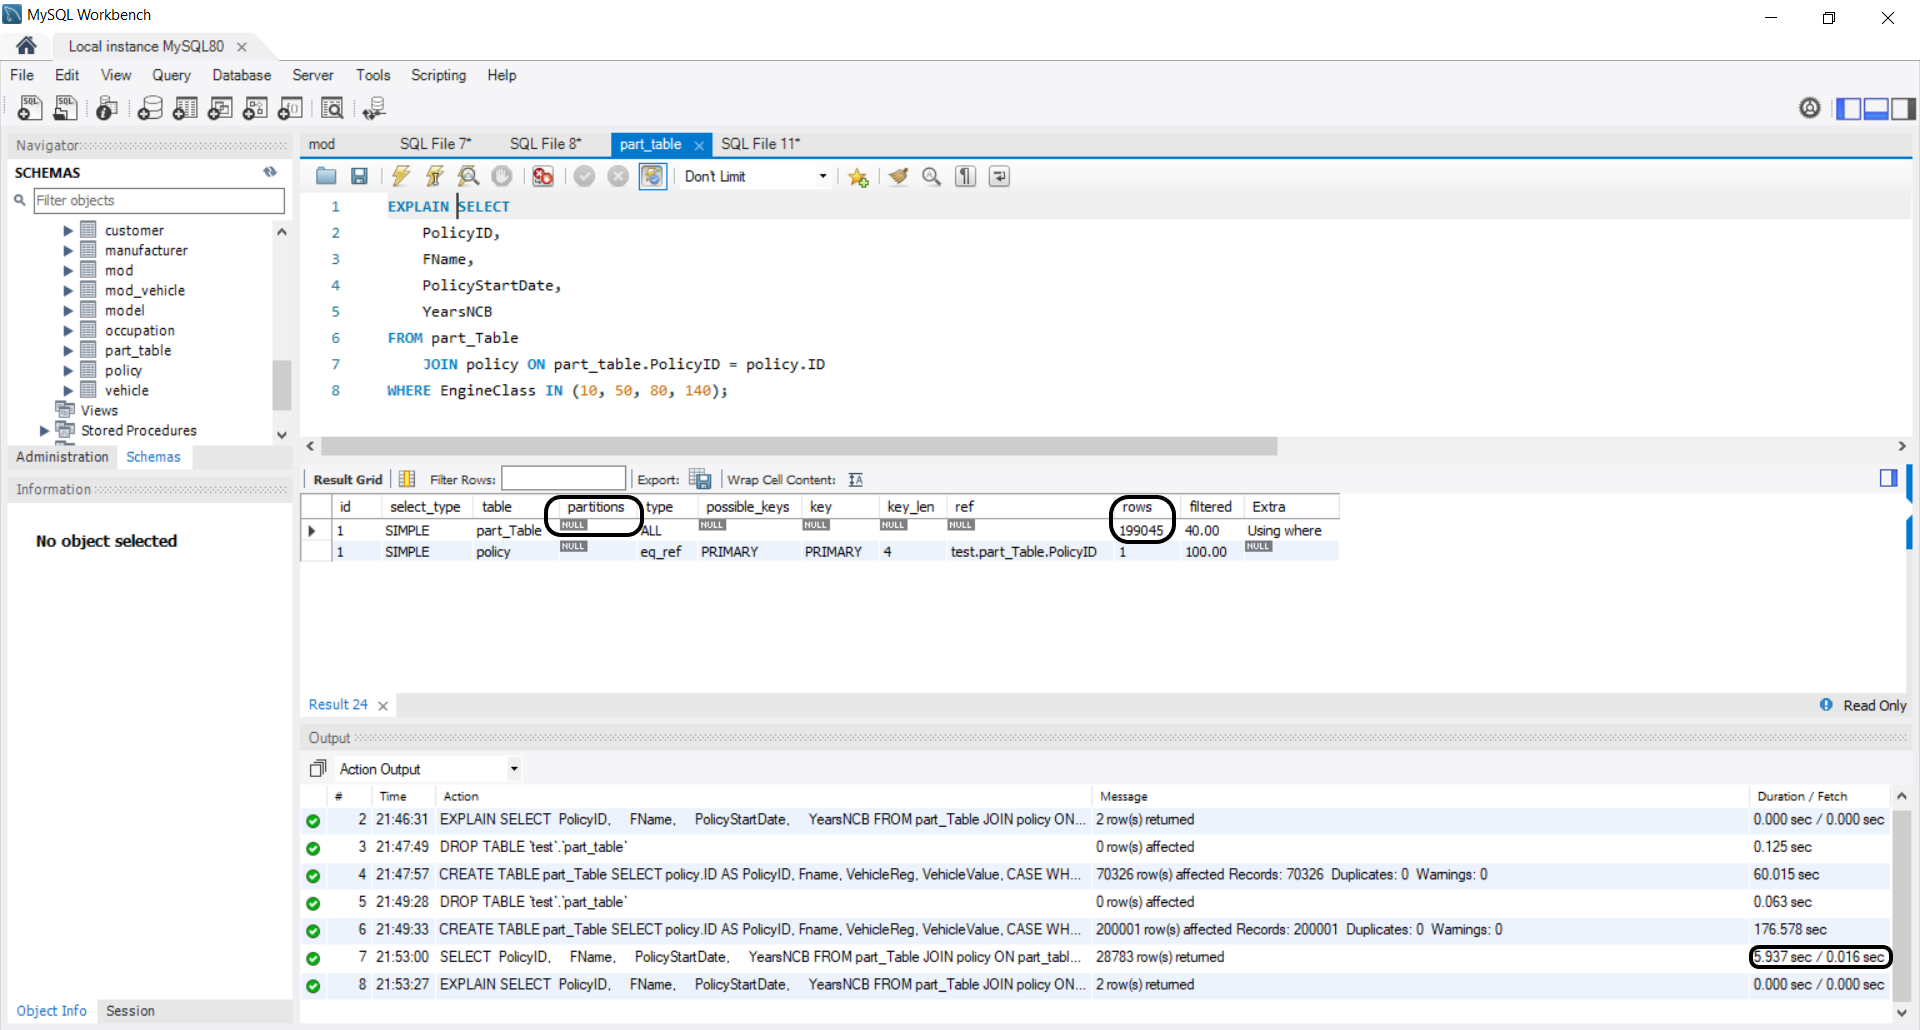
\includegraphics[width=\linewidth]{Before}
	
	{\bf Sau khi thêm partition:}
	\\
	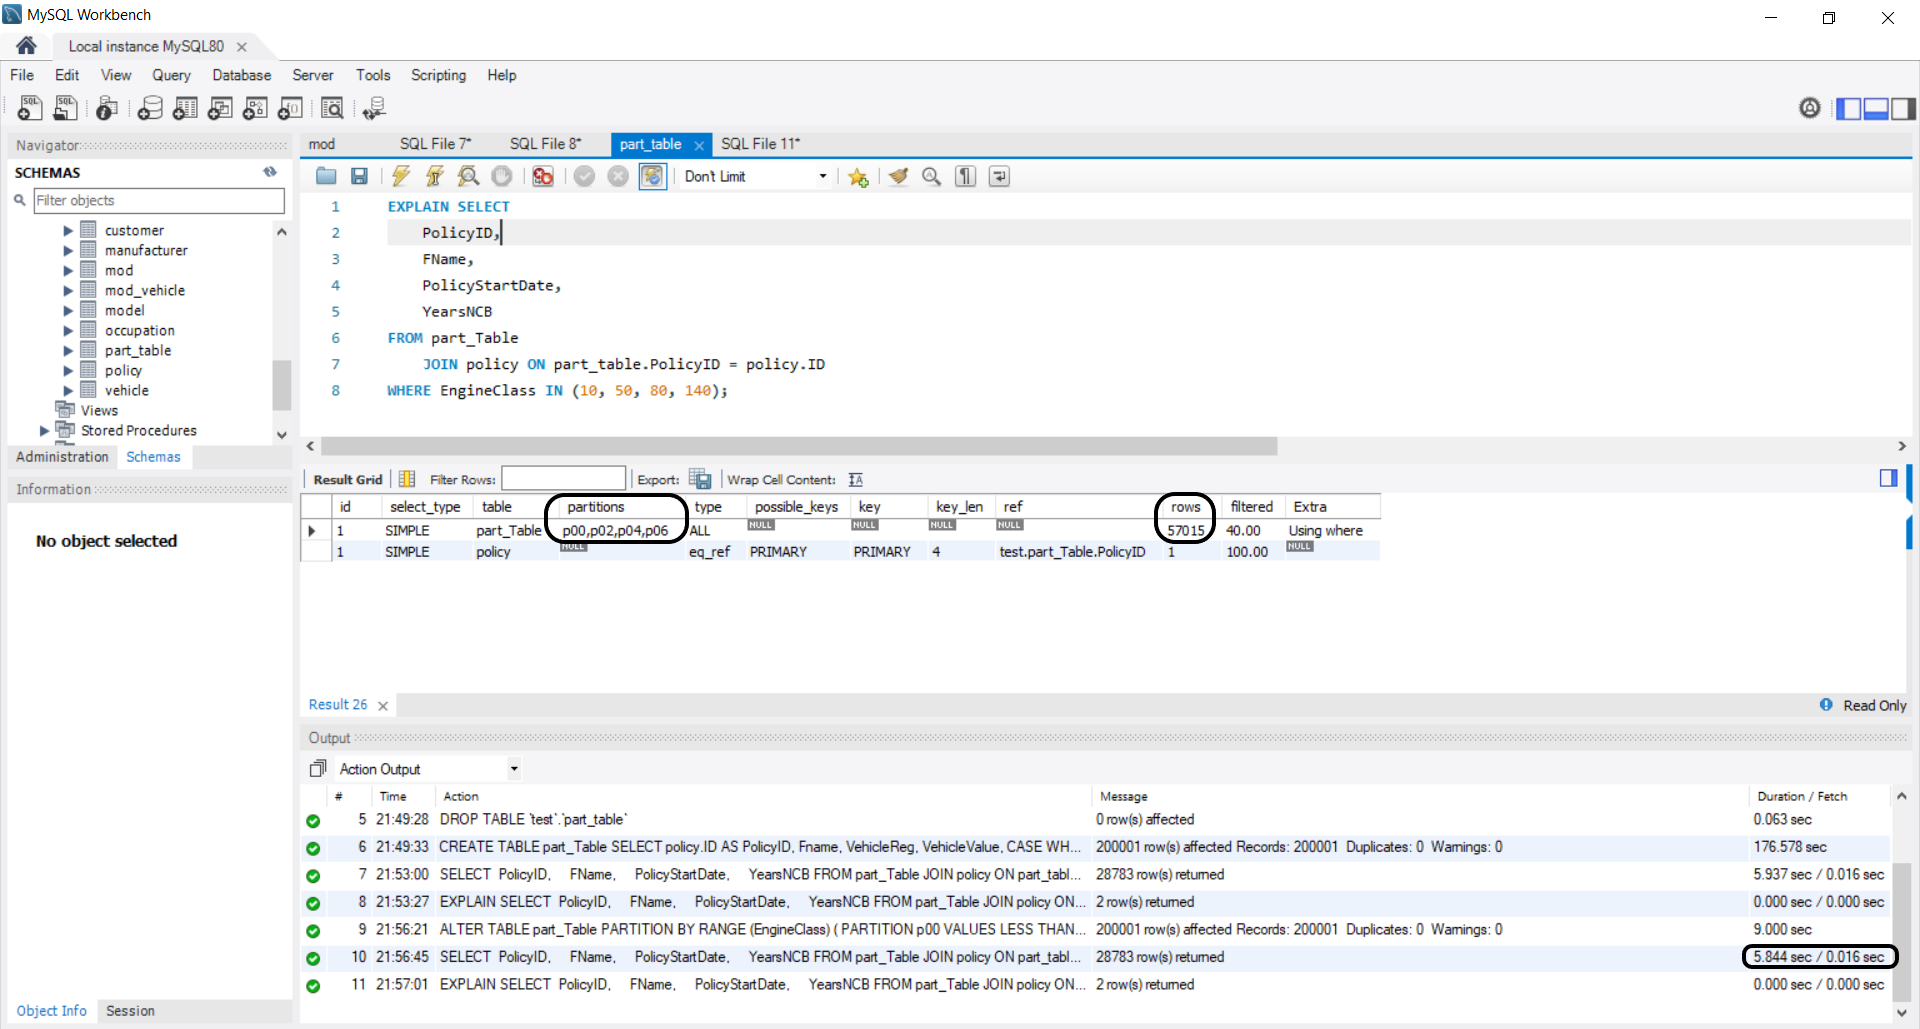
\includegraphics[width=\linewidth]{After}























\end{document}